\section{Inventory Characterization}
\label{sec:results-baseline}

Before any transmutation results are presented, this section characterizes the
inventory that the \texttt{us\_inventory} archetype ingests, establishing both
that the \gls{STANDARDS}~5.0.1 dataset is loaded correctly and the scale and
distribution of the material available to the fuel cycle. Because the inventory
load is deterministic, the same directory of assembly records always produces
the same pool, these results depend only on the input data and the parser, not
on any simulation dynamics.

Reading the 75 assembly-record files yields $315{,}976$ individual assemblies,
totalling $8.69\times10^{4}~\mathrm{t}$ of heavy metal, drawn from 61 facilities
for which geographic coordinates are available. Summing the minor-actinide
content of every assembly, as defined in Equation~\ref{eq:usinv-ma-fraction},
gives a total accessible minor-actinide inventory of $103.8~\mathrm{t}$. This
minor actinide is only $0.12\%$ of the total heavy metal, a consequence of the
low neptunium, americium, and curium content of discharged
light-water-reactor fuel. Put in terms of the burner, the entire national
minor-actinide inventory amounts to fewer than four \gls{ADS} cores at the
$27~\mathrm{t}$ core loading of the minor-actinide-only case
(Table~\ref{tab:scenario-config}). This scarcity is the central constraint on
the transmutation mission and recurs throughout the results: the burner is
limited far more by the availability of minor actinide than by any reactor
parameter.

Figure~\ref{fig:results-source-map} shows the geographic distribution of this
material, with each facility placed at its coordinates and shaded by the mass of
spent fuel it supplies over a full-horizon run. Because the run draws down the
accessible inventory, the drawn mass approaches the available inventory at each
site, so the figure doubles as a map of where the national inventory resides.
The distribution is strongly weighted toward the eastern and south-central
United States, where the largest single sites each supply on the order of
$2{,}500$--$2{,}700~\mathrm{t}$, while the smaller western sites contribute a few
hundred tonnes. This spatial concentration is the starting point for the
provenance analysis of Section~\ref{sec:results-policy}, since any policy that
draws assemblies in a particular order also implies a particular geographic
sequence of retrieval.

\begin{figure}[htbp]
  \centering
  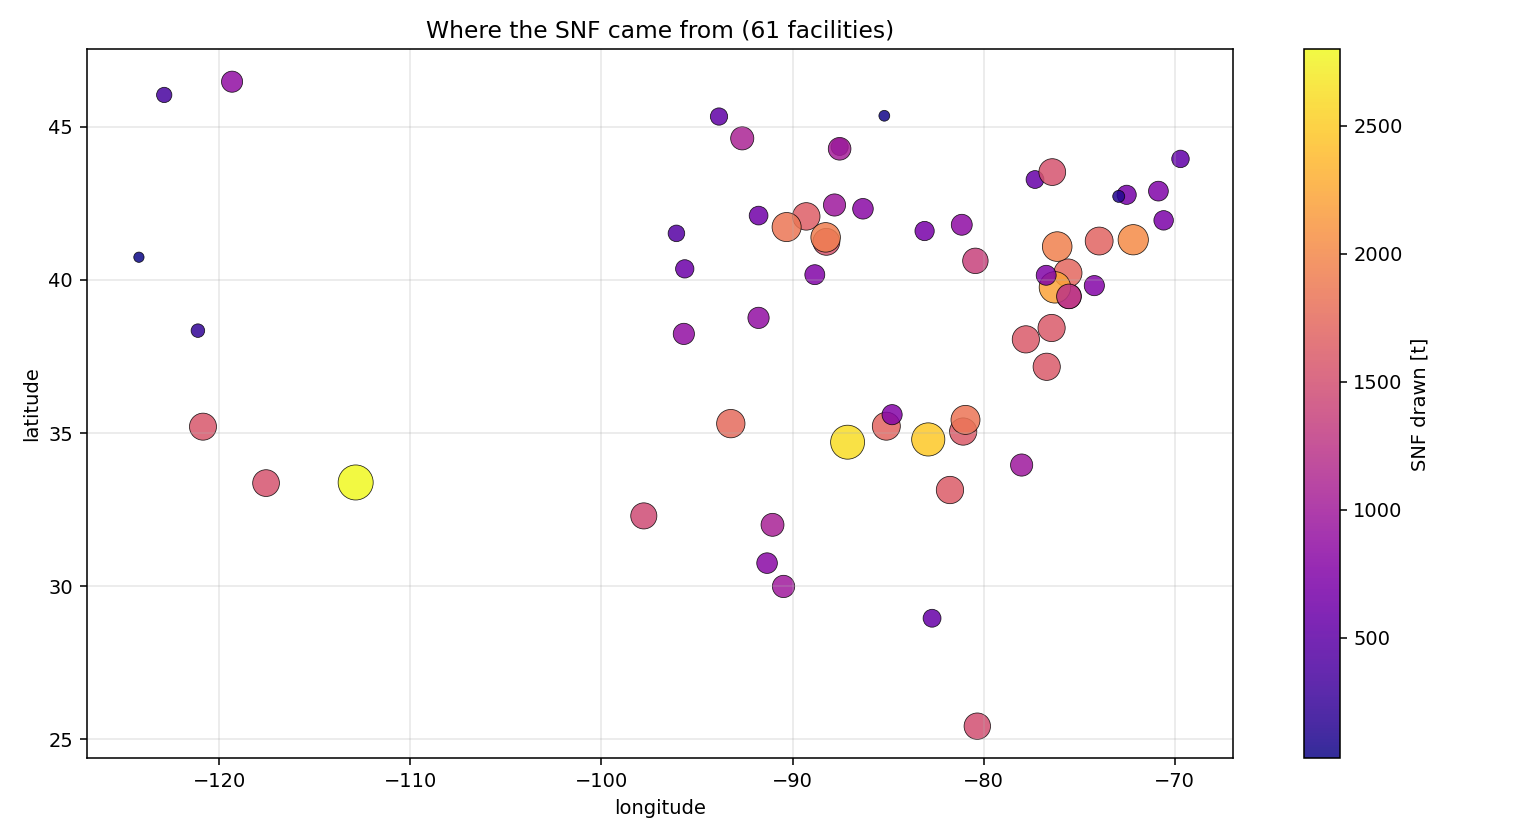
\includegraphics[width=0.95\textwidth]{figures/results_source_map}
  \caption[Geographic distribution of the sourced U.S.\ spent-fuel
  inventory.]{Geographic distribution of the spent nuclear fuel supplied by the
  \texttt{us\_inventory} archetype. Each marker is one of the 61 facilities with
  known coordinates, positioned by latitude and longitude and shaded and sized
  by the mass of spent fuel drawn over the full simulation horizon. The
  inventory is concentrated in the eastern and south-central United States.}
  \label{fig:results-source-map}
\end{figure}

Establishing this baseline confirms that the archetype ingests the assembly-level
dataset faithfully and quantifies the material the transmutation fuel cycle has
to work with. The remainder of this chapter examines how that material is
selected (Section~\ref{sec:results-policy}), how it is transmuted in the
\gls{ADS} (Section~\ref{sec:results-ads}), and how the accessible inventory
evolves under recycling (Section~\ref{sec:results-evolution}).

%%%%%%%%%%%%%%%%%%%%%%%%%%%%%%%%%%%%%%%%%%%%%%%%%%%%%%%%%%%%%%%%%%%%%%%%%%%%%%%%%%%%%%%%%%%%%%%%%%%%%%%%%%%%%%%%%%%%%%%%%%%%%%%%%
%%%%%%%%%%%%%%%%%%%%%%%%%%%%%%%%%%%%%%%%%%%%%%%%%%%%%%%%%%%%%%%%%%%%%%%%%%%%%%%%%%%%%%%%%%%%%%%%%%%%%%%%%%%%%%%%%%%%%%%%%%%%%%%%%
%%%%%%%%%%%%%%%%%%%%%%%%%%%%%%%%%%%%%%%%%%%%%%%%%%%%%%%%%%%%%%%%%%%%%%%%%%%%%%%%%%%%%%%%%%%%%%%%%%%%%%%%%%%%%%%%%%%%%%%%%%%%%%%%%

\section{Effect of Selection Policy on the Feed}
\label{sec:results-policy}

The \texttt{us\_inventory} archetype selects individual assemblies by an explicit
ranking policy (Section~\ref{subsec:us-inventory-policies}), and that choice
determines the mass and composition of material delivered to separations and,
ultimately, to the burner. The selection mechanism acts on the static inventory
pool and is deterministic in the assembly ordering it produces: it does not
depend on downstream reactor dynamics. Its effect on the feed can therefore be
characterized directly, from the inventory data and from standalone
\texttt{us\_inventory} runs, independently of the full fuel cycle, and that is
how it is presented in this section. The production scenarios of
Chapter~\ref{ch:results} all use \texttt{highest\_minor\_actinide}
(Section~\ref{subsec:scenario-flowsheet}); the comparisons here show what that
choice buys relative to the alternatives.

\subsection{Delivery Trajectory}
\label{subsec:results-policy-trajectory}

Because every policy eventually draws from the same finite pool, the total
minor actinide any policy can deliver is identical: the cumulative curves all
terminate at the same $103.8~\mathrm{t}$
(Section~\ref{sec:results-baseline}). What the policy changes is the
\emph{trajectory}, how quickly minor actinide accumulates as assemblies are
drawn. Figure~\ref{fig:results-policy-trajectory} shows the cumulative minor
actinide delivered against the number of assemblies drawn, for the three
representative policies of set~A, with a horizontal line marking one
$27~\mathrm{t}$ minor-actinide-only core.

The separation is large. Ranking by \texttt{highest\_minor\_actinide} reaches a
full core after roughly $4.8\times10^{4}$ assembly draws, whereas
\texttt{lowest\_minor\_actinide} requires about $1.28\times10^{5}$, a factor of
$2.7$ more material handled for the same core. The unranked \texttt{first}
baseline falls between them, at about $7.7\times10^{4}$ draws, and its curve is
visibly segmented: because \texttt{first} draws facility by facility in load
order, its slope steps up and down as it moves through sites of differing minor-
actinide quality, whereas the ranked policies produce smooth, monotonically
curving trajectories. The timing here is expressed in assemblies drawn rather
than calendar time, since the mapping to time depends on the per-step retrieval
throughput, which is not the subject of this comparison.

This is the practical face of the scarcity established in
Section~\ref{sec:results-baseline}. With the national inventory holding fewer
than four cores of minor actinide in total, the order of retrieval governs how
much spent fuel must be handled, and, as shown next, from how many sites, to
assemble even a single core.

\begin{figure}[htbp]
  \centering
  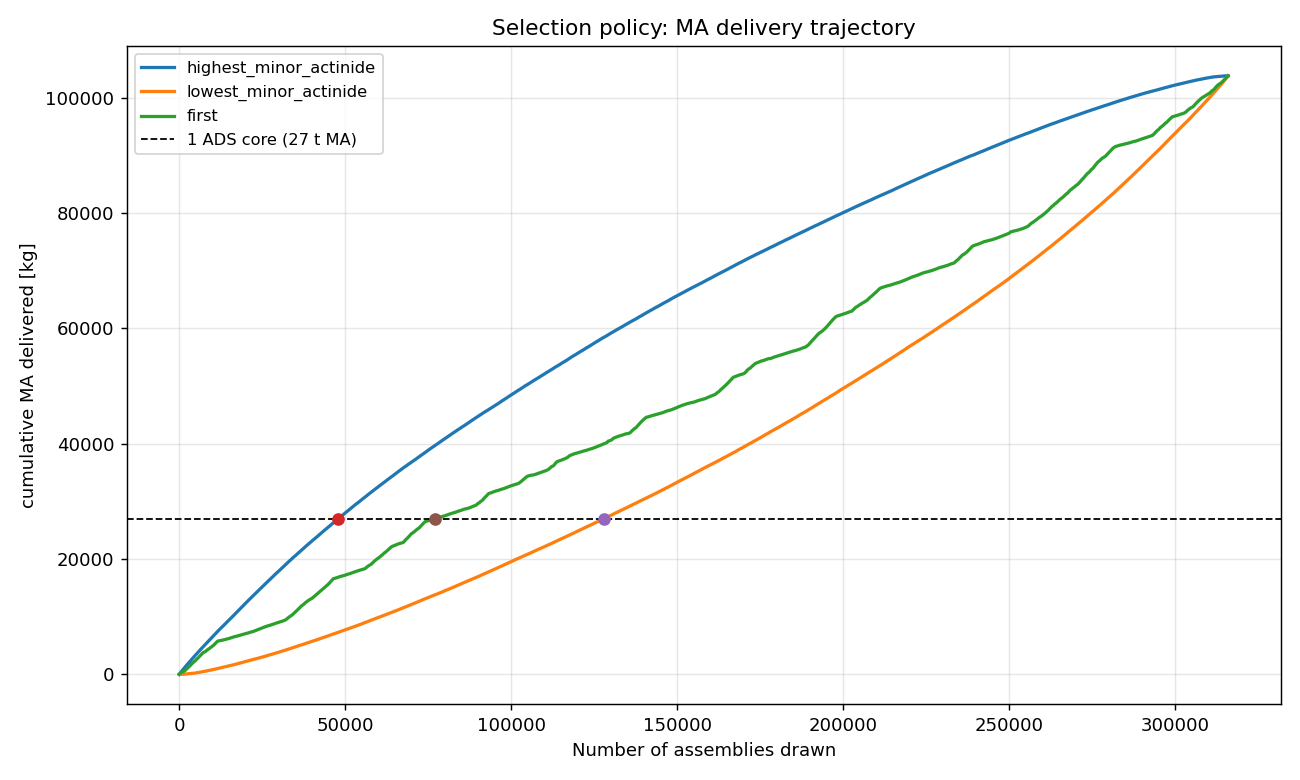
\includegraphics[width=0.9\textwidth]{figures/policy_trajectory}
  \caption[Minor-actinide delivery trajectory by selection policy.]{Cumulative
  minor actinide delivered as a function of assemblies drawn, for three
  selection policies. All policies terminate at the same total, since they draw
  from one finite pool; they differ only in how quickly minor actinide
  accumulates. The dashed line marks one $27~\mathrm{t}$ minor-actinide-only
  core; markers indicate where each policy first supplies a full core.
  \texttt{highest\_minor\_actinide} reaches a core with roughly $2.7$ times
  fewer draws than \texttt{lowest\_minor\_actinide}.}
  \label{fig:results-policy-trajectory}
\end{figure}

\subsection{Geographic Provenance of the Feed}
\label{subsec:results-policy-provenance}

Because the selection order is also a geographic order, each policy implies a
different set of sites supplying the first core.
Figure~\ref{fig:results-policy-provenance} shows the minor actinide contributed
by each facility to the first $27~\mathrm{t}$ core under the set~A policies.
The contrast is stark. The \texttt{first} policy, drawing in load order,
concentrates the core in a handful of sites, each contributing on the order of
$2~\mathrm{t}$; \texttt{highest\_minor\_actinide} instead spreads the draw across
many facilities, tapping the minor-actinide-rich assemblies wherever they
reside, so that no single site dominates. Ranking for feed quality thus trades a
geographically concentrated retrieval for a distributed one, a consideration
that connects directly to transportation and logistics, which fall outside the
scope of this work but are enabled by the provenance recorded in
\texttt{us\_inventorySupply} (Table~\ref{tab:usinv-supply}).

\begin{figure}[htbp]
  \centering
  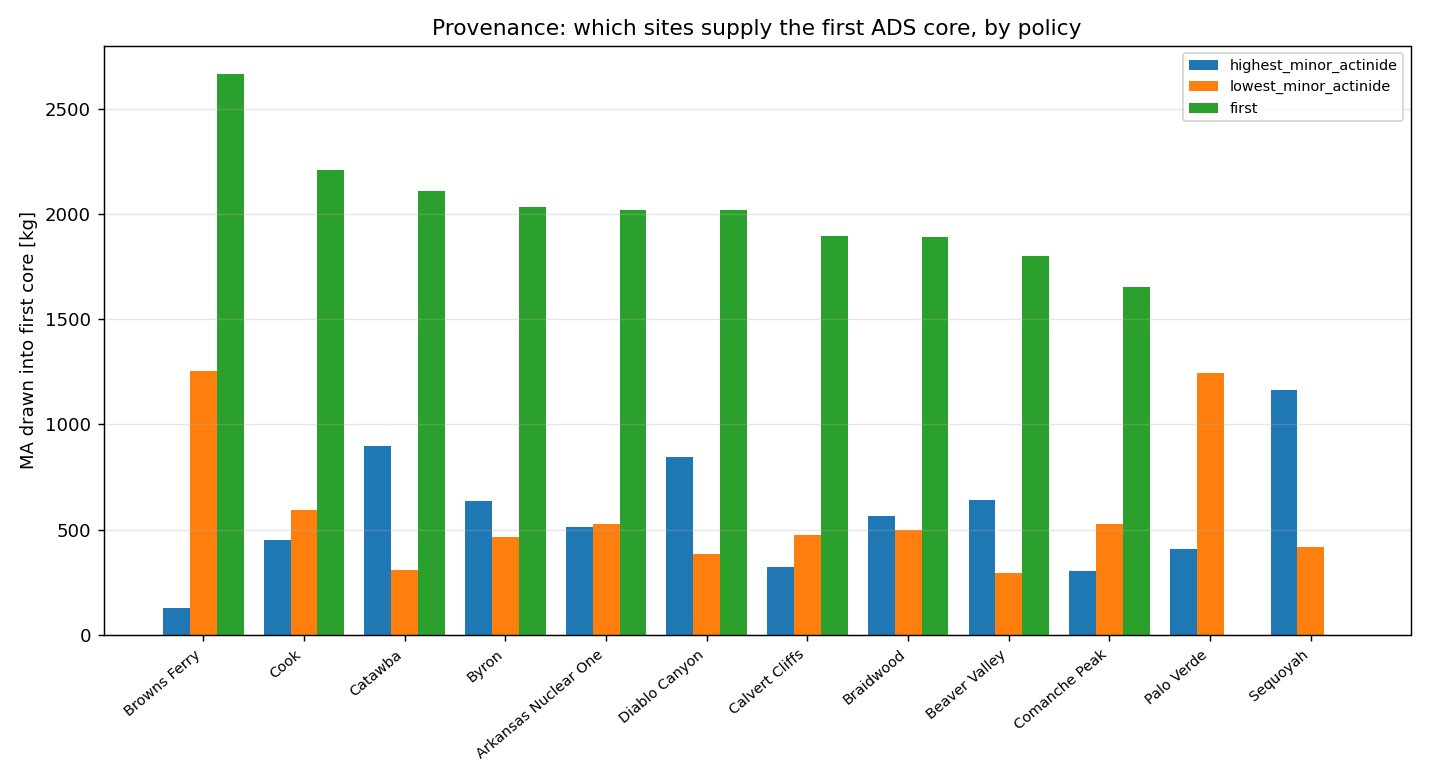
\includegraphics[width=0.95\textwidth]{figures/policy_provenance}
  \caption[Facility provenance of the first core by selection policy.]{Minor
  actinide contributed by each facility to the first $27~\mathrm{t}$ core, for
  the set~A policies. \texttt{first} concentrates the core in a few sites drawn
  in load order, while \texttt{highest\_minor\_actinide} distributes it across
  many facilities.}
  \label{fig:results-policy-provenance}
\end{figure}

The effect is not specific to minor-actinide ranking. When the pool is instead
ordered by discharge age (\texttt{older}, \texttt{newer}) or by reported burnup
(\texttt{highest\_burnup}, \texttt{lowest\_burnup}), the set of sites supplying
the first core shifts again, each policy favoring the facilities whose
assemblies rank highest under its criterion. This confirms that the archetype's
selection acts as a general lever on feed provenance: any physical property
recorded in the assembly data can be used to reshape both the composition and
the geographic origin of the material entering the fuel cycle.

Finally, that the mechanism operates identically inside a full \Cyclus
simulation, not only in offline analysis of the pool, was confirmed in a
standalone \texttt{us\_inventory} run in which the average composition of the
supplied material tracked the active policy, with plutonium- and
burnup-ranked policies delivering the correspondingly higher plutonium and
fissile fractions expected from the ranking.


%%%%%%%%%%%%%%%%%%%%%%%%%%%%%%%%%%%%%%%%%%%%%%%%%%%%%%%%%%%%%%%%%%%%%%%%%%%%%%%%%%%%%%%%%%%%%%%%%%%%%%%%%%%%%%%%%%%%%%%%%%%%%%%%%
%%%%%%%%%%%%%%%%%%%%%%%%%%%%%%%%%%%%%%%%%%%%%%%%%%%%%%%%%%%%%%%%%%%%%%%%%%%%%%%%%%%%%%%%%%%%%%%%%%%%%%%%%%%%%%%%%%%%%%%%%%%%%%%%%
%%%%%%%%%%%%%%%%%%%%%%%%%%%%%%%%%%%%%%%%%%%%%%%%%%%%%%%%%%%%%%%%%%%%%%%%%%%%%%%%%%%%%%%%%%%%%%%%%%%%%%%%%%%%%%%%%%%%%%%%%%%%%%%%%

\section{ADS Transmutation Performance}
\label{sec:results-ads}

This section examines how the \gls{ADS} transmutes the separated feed. Of the
eight runs defined in Section~\ref{subsec:scenario-runs}, most coincide: as
anticipated there, the once-through and recycling modes produce nearly identical
histories wherever the burner is cycle-limited rather than feed-limited, so a
single representative run suffices for those cases. The results therefore reduce
to two comparisons that isolate the physics of interest. The first contrasts the
two burner configurations, the minor-actinide-only core (ADS~1) and the
\(50/50\) plutonium-minor-actinide core (ADS~2), over the 100-year horizon,
establishing how core size and feed composition govern the burner's behavior. The
second contrasts recycling against once-through operation for the
minor-actinide-only core, the one pairing where the two modes diverge. Throughout,
the per-cycle transmutation physics is identical between modes and horizons; what
changes is how many cycles the burner completes before it exhausts its feed.

\subsection{Per-Cycle Transmutation and Burn Fraction}
\label{subsec:results-ads-burn}

At each discharge the core composition is read from the matched \textsc{Serpent}
case (Section~\ref{subsec:ads-discharge}), giving the surviving actinides and the
fission products produced during the cycle. Figures~\ref{fig:results-case3-recycle-fpyield}
and~\ref{fig:results-case4-recycle-fpyield} show the cumulative fission-product
yield of the two cores, plotted against fission-product mass number. Both are the
familiar double-humped curve of low-to-moderate-energy actinide fission, with a
light peak near \(A \approx 100\) and a heavy peak near \(A \approx 138\)
separated by the symmetric-fission valley. For the minor-actinide-only core
(Figure~\ref{fig:results-case3-recycle-fpyield}) this signature appears even though
the feed contains no uranium or plutonium, confirming that the minor actinides
themselves are fissioning in the fast, subcritical core: the double hump is a
property of the fission fragments' shell structure, not of which actinide split.
In both cases the three burnup snapshots nearly overlie one another, since the
cumulative yield shape is set by the actinide mixture, which shifts only slowly
with irradiation.

The two cores differ in the details of the distribution, and the difference
reflects their feed. The \(50/50\) core
(Figure~\ref{fig:results-case4-recycle-fpyield}) contains a large plutonium
fraction, and \({}^{239}\mathrm{Pu}\) fissions from a heavier compound nucleus
than the minor-actinide vector; heavier fissioning systems place the light peak
slightly higher in mass and fill in the symmetric valley, reducing the
peak-to-valley ratio. The minor-actinide-only core, fissioning a lighter mix
dominated by americium and neptunium, is consistent with a marginally deeper
valley and a light peak shifted slightly lower. The shift is subtle because both
feeds fission in the same fast spectrum and span overlapping actinide masses, but
it is the expected signature of a plutonium-bearing versus a plutonium-free feed,
and it confirms that the reduced-order model carries the compositional distinction
through to the fission-product inventory.

\begin{figure}[htbp]
  \centering
  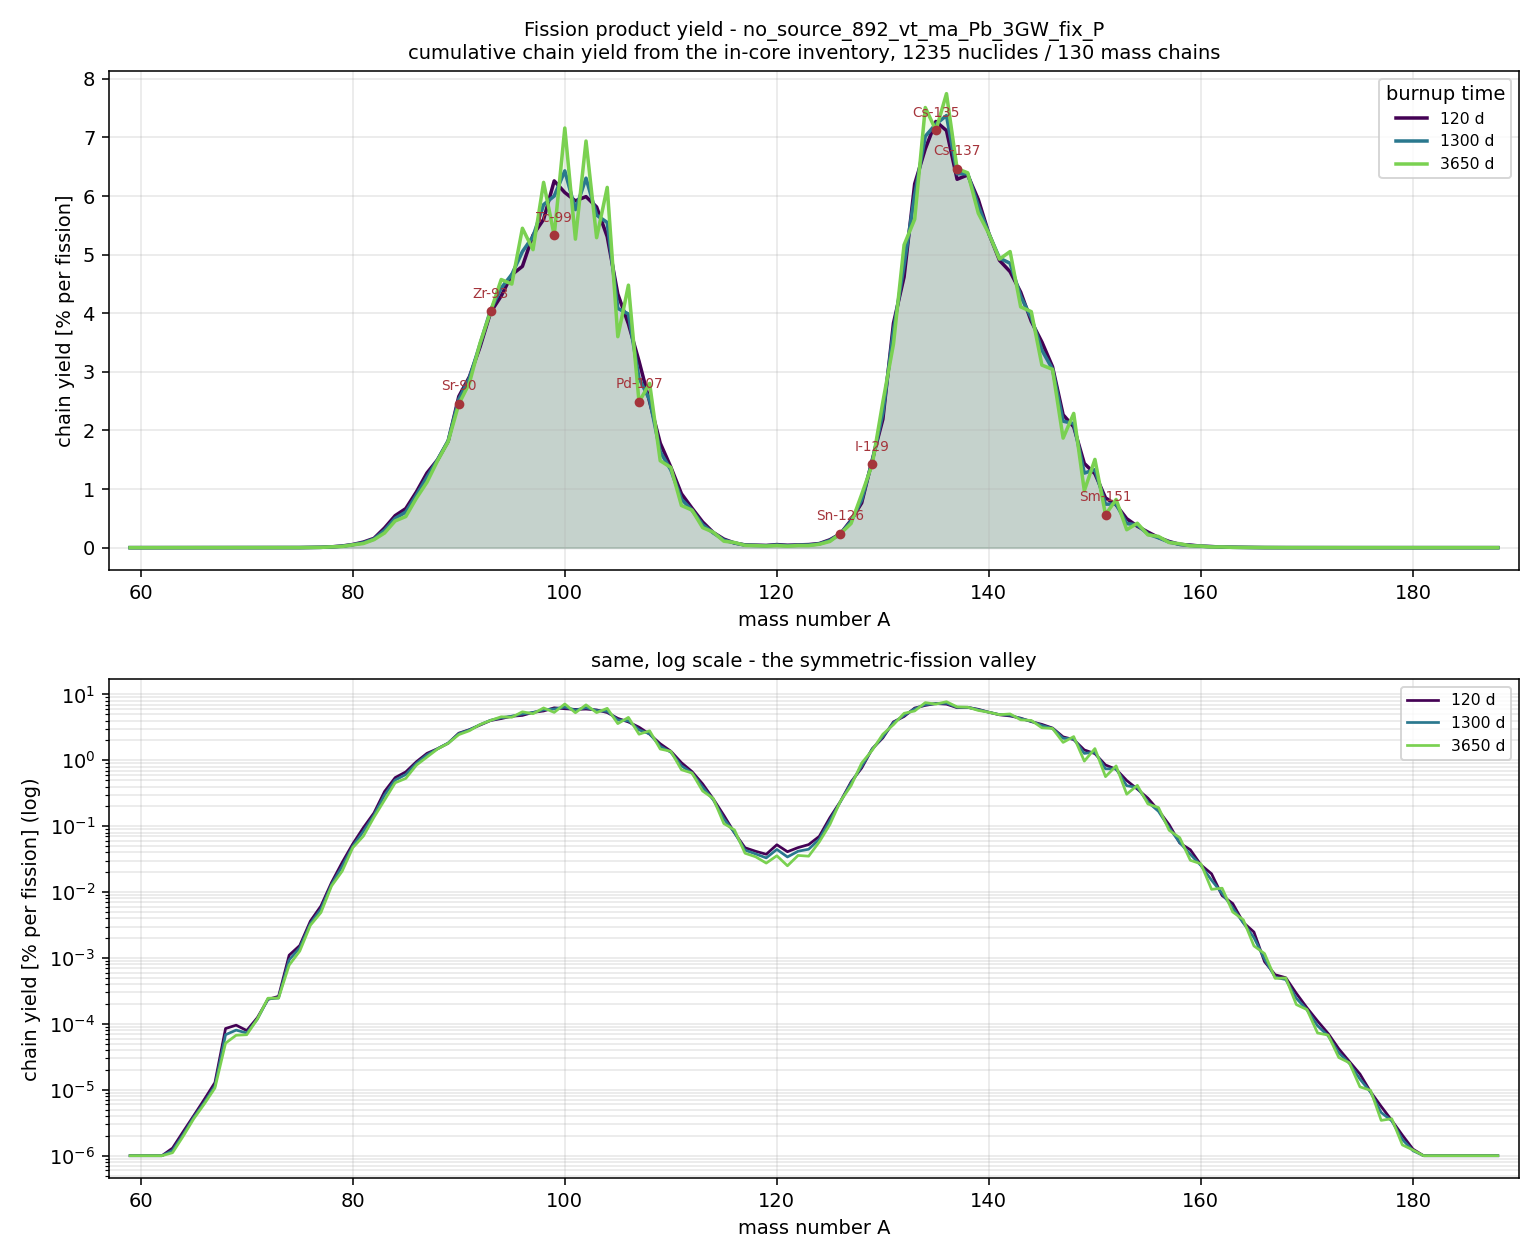
\includegraphics[width=0.9\textwidth]{figures/case3_ma_recycle_100yr_fp_yield}
  \caption[Fission-product yield of the minor-actinide-only core.]{Cumulative
  fission-product chain yield of the minor-actinide-only core (ADS~1) as a
  function of fission-product mass number, at three points in the irradiation. The
  double-humped distribution appears despite the absence of uranium or plutonium
  in the feed, confirming that the minor actinides are the fissioning species.}
  \label{fig:results-case3-recycle-fpyield}
\end{figure}

\begin{figure}[htbp]
  \centering
  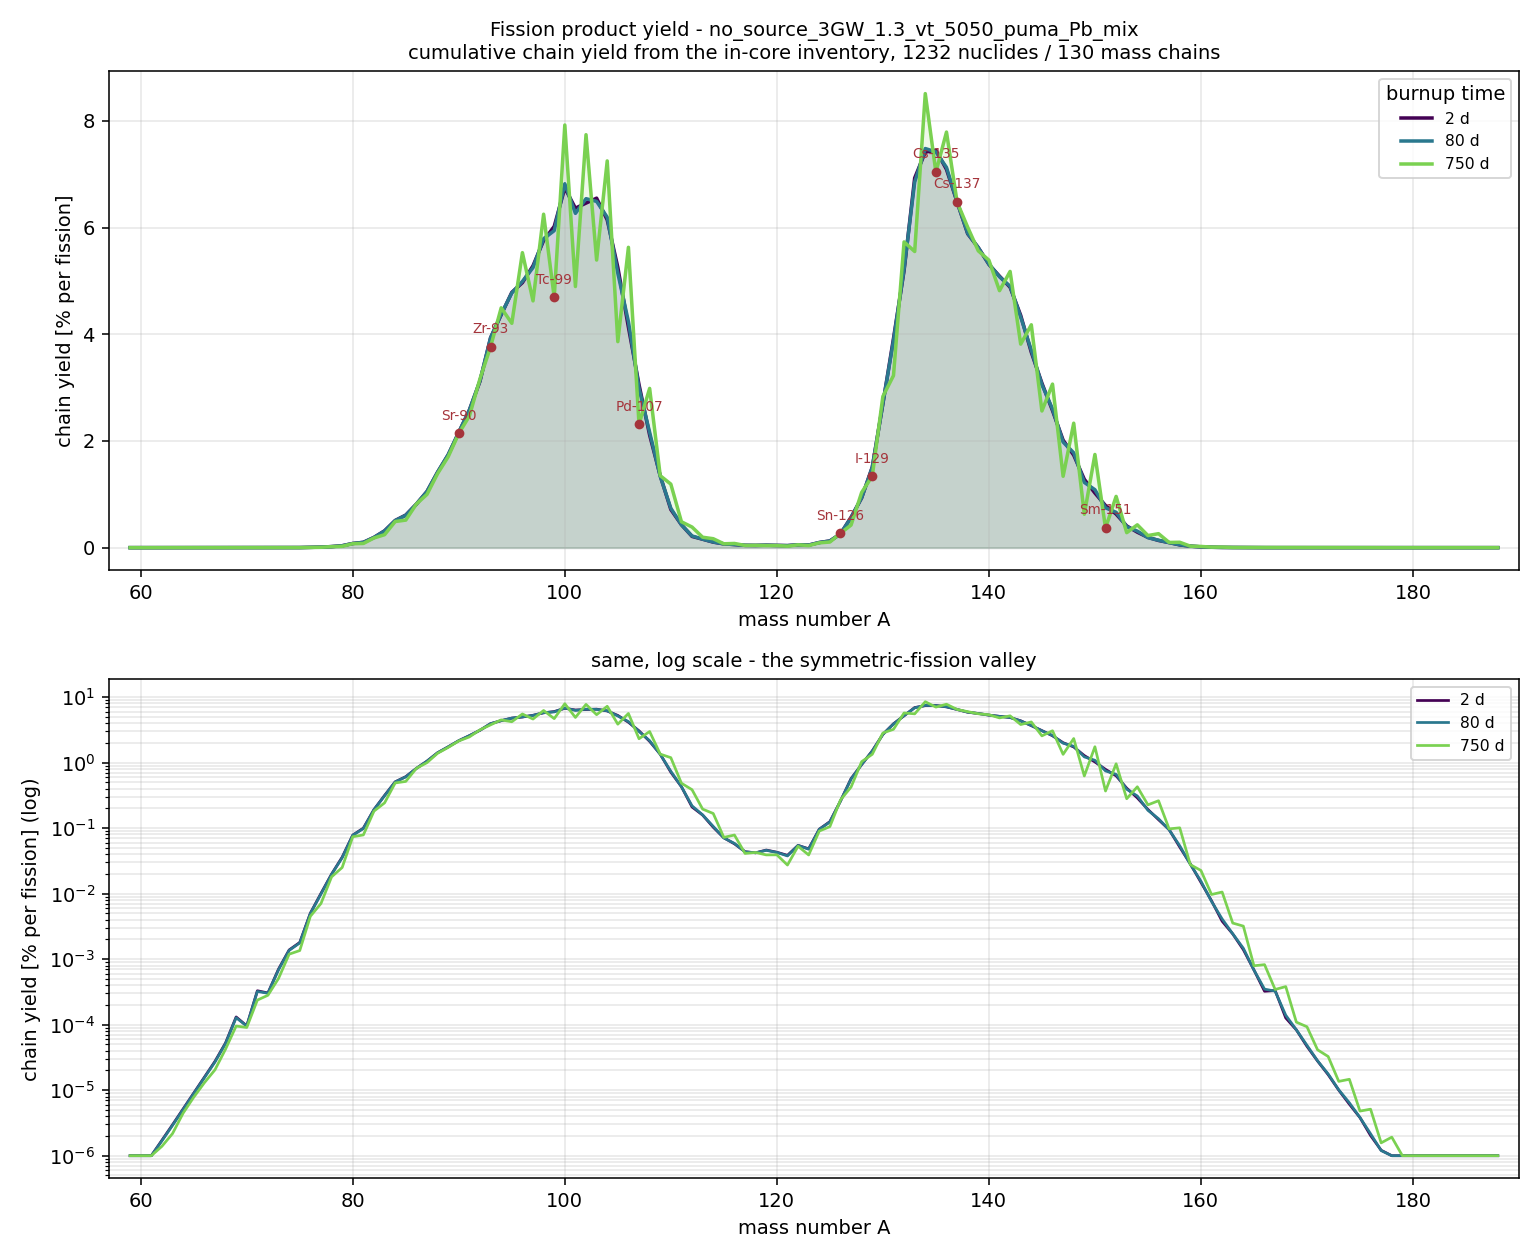
\includegraphics[width=0.9\textwidth]{figures/case4_puma_recycle_100yr_fp_yield}
  \caption[Fission-product yield of the \(50/50\) core.]{Cumulative fission-product
  chain yield of the \(50/50\) plutonium-minor-actinide core (ADS~2). Relative to
  the minor-actinide-only core, the plutonium-bearing feed fills in the
  symmetric-fission valley and shifts the light peak slightly higher in mass, the
  expected signature of a heavier fissioning system.}
  \label{fig:results-case4-recycle-fpyield}
\end{figure}

The per-cycle mass accounting is summarized by the burn fraction, the ratio of
actinide mass destroyed to actinide mass charged. For the minor-actinide-only
core this fraction is constant at \(41.3\%\) across every cycle
(Figure~\ref{fig:results-case3-recycle-percycle}), a direct consequence of the
reduced-order model: each core is irradiated to the same point on the same
depletion trajectory, so each cycle removes the same fraction of its charge. For
the \(50/50\) core the burn fraction rises to just under \(50\%\)
(Figure~\ref{fig:results-case4-recycle-percycle}); the plutonium half of that feed
fissions more readily than the minor-actinide vector, so a larger fraction of each
charge is consumed per pass.

The burn fraction reported here is the net reduction in total actinide mass,
calculated from the \texttt{ActinideDestroyed} event according to
Equation~\ref{eq:ads-destroyed}. Equation~\ref{eq:ads-ratio} first determines the
mass retained in the discharged product, after which the archetype subtracts the
total actinide mass remaining in that product from the total actinide mass in the
matched case's initial loading. Because plutonium is included in the total
actinide inventory, minor actinides converted into plutonium remain in
\(M_{\mathrm{out}}a_c(t_{\mathrm{irr}})\) and are not counted as destroyed. The
reported value therefore represents net actinide destruction in the tracked
depletion inventory, rather than the disappearance of minor actinides alone.

This per-cycle rate can be checked against first principles. Fissioning one
kilogram of actinide releases approximately \(0.93~\mathrm{GW\text{-}d}\) of
thermal energy, so a \(3000~\mathrm{MW_{th}}\) core destroys about
\(3.2~\mathrm{kg}\) of actinide per full-power day, or roughly
\(1{,}120~\mathrm{kg\,yr^{-1}}\) at full power. Applied to the ten-year
minor-actinide cycle, this predicts a per-cycle destruction close to the
\(11{,}150~\mathrm{kg}\) read from the \textsc{Serpent} case, agreeing to within a
few percent. The reduced-order transmutation model is therefore consistent with
the fission energy balance, an independent validation of the archetype's mass
accounting.

\begin{figure}[htbp]
  \centering
  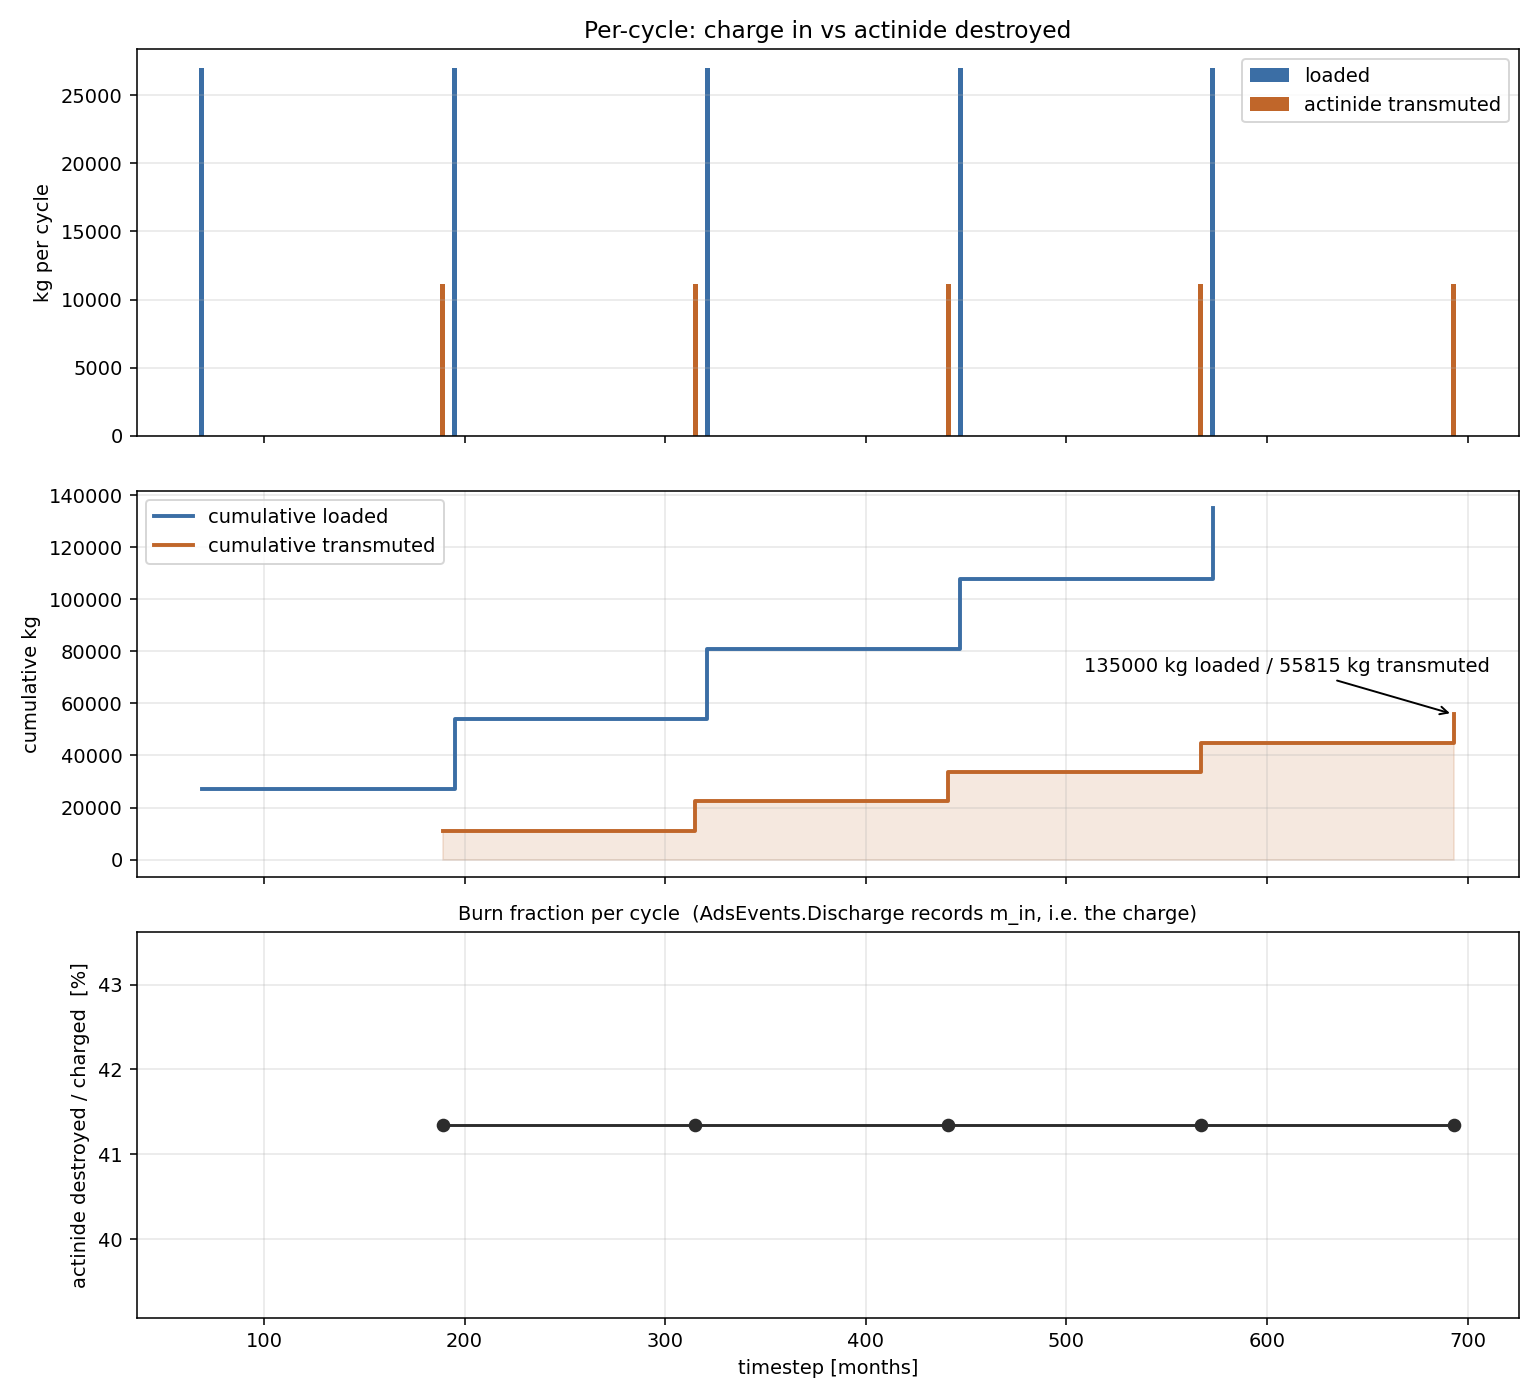
\includegraphics[width=0.95\textwidth]{figures/case3_ma_recycle_100yr_percycle}
  \caption[Per-cycle mass accounting for the minor-actinide-only core.]{Per-cycle
  charge and actinide destruction for the minor-actinide-only core (ADS~1),
  100-year recycling run. Each cycle charges \(27~\mathrm{t}\) and records
  \(11.15~\mathrm{t}\) of net actinide destruction, a constant burn fraction of \(41.3\%\) (bottom panel). The
  cumulative panel (centre) reaches \(135~\mathrm{t}\) charged and
  \(55.8~\mathrm{t}\) of cumulative net actinide destruction over five cycles.}
  \label{fig:results-case3-recycle-percycle}
\end{figure}

\begin{figure}[htbp]
  \centering
  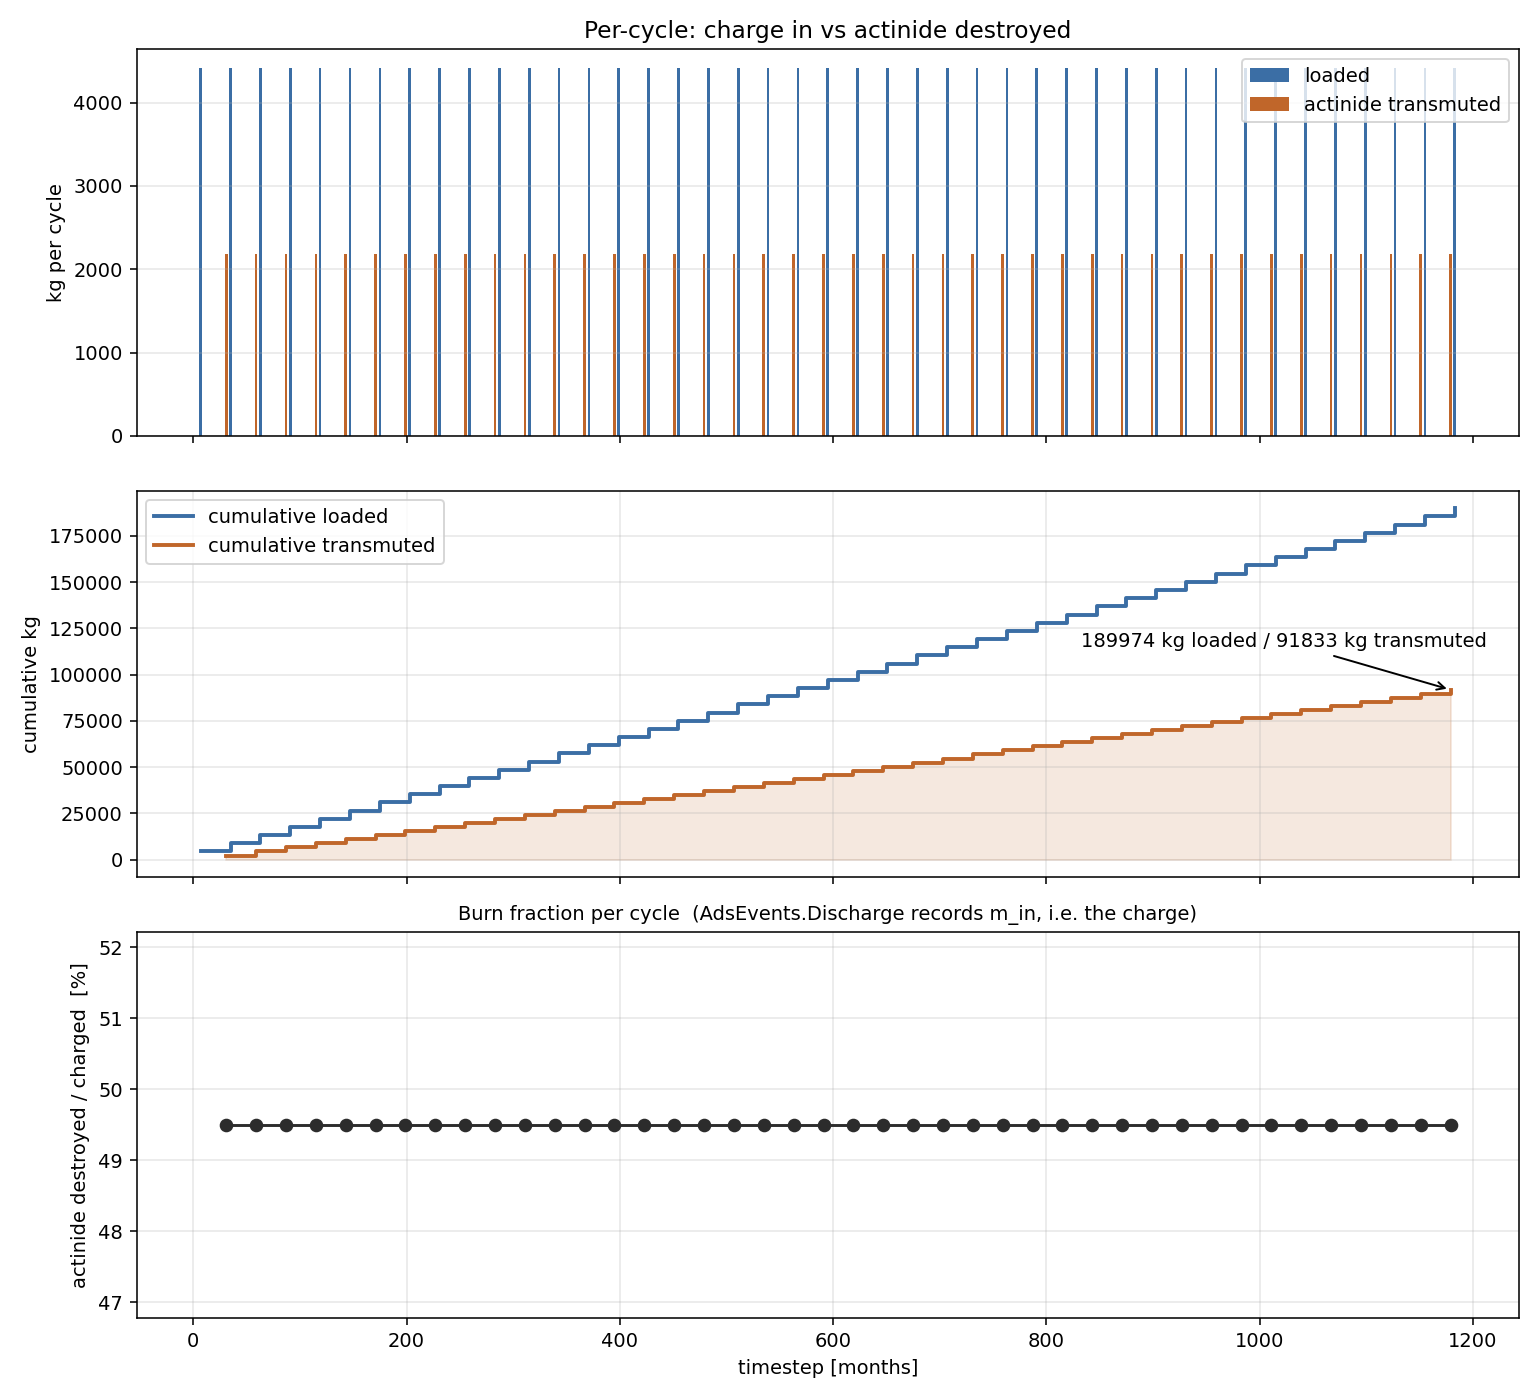
\includegraphics[width=0.95\textwidth]{figures/case4_puma_recycle_100yr_percycle}
  \caption[Per-cycle mass accounting for the \(50/50\) core.]{Per-cycle charge and
  actinide destruction for the \(50/50\) plutonium-minor-actinide core (ADS~2),
  100-year recycling run. Each cycle charges \(4.4~\mathrm{t}\) and records
  \(2.2~\mathrm{t}\) of net actinide destruction, a burn fraction just under \(50\%\). The small, fast-cycling
  core completes 42 cycles over the horizon.}
  \label{fig:results-case4-recycle-percycle}
\end{figure}

\subsection{Core Size and Feed Composition: the Two Burner Cases}
\label{subsec:results-ads-cases}

The two burner configurations produce very different operating histories, driven
entirely by core size and the resulting cycle length.
Figures~\ref{fig:results-case3-recycle-dutycycle}
and~\ref{fig:results-case4-recycle-dutycycle} show the core state, irradiating or
idle, over the 100-year horizon for the two cases.

The minor-actinide-only core is large (\(27~\mathrm{t}\)) and is irradiated for
ten years per cycle. Over 100 years of recycling it completes only five cycles and
then falls idle for the remainder of the horizon, reaching a duty factor of
\(50\%\). The core stops not because the horizon ends, but because the quantity
of recoverable neptunium, americium, and curium accumulated in its feed buffer no
longer reaches the \(27~\mathrm{t}\) full-core loading required by the archetype.
This does not mean that no actinide remains in the fuel cycle: some surviving
actinide has been converted to plutonium, which is not returned to the
minor-actinide-only feed, while additional material remains in discharged
products, waste, and facility buffers. The \(50/50\) core, by contrast, is small
(\(4.4~\mathrm{t}\)) and is cycled every two years. It completes 42 cycles and
runs essentially continuously across the full horizon, at a duty factor of
\(85\%\). It never exhausts its feed because it consumes minor actinide slowly and
supplements it with the far more abundant plutonium.

This is the central distinction between the two configurations. The
minor-actinide-only core is \emph{feed-limited}: its throughput is set by how much
minor actinide the inventory can supply, not by reactor physics. The \(50/50\)
core is \emph{cycle-limited}: it processes feed as fast as its cycle allows, and
the inventory is deep enough, because it draws on plutonium, to sustain that pace
for a century. The trade-off is that the \(50/50\) core is no longer a pure
minor-actinide burner: half of what it destroys is plutonium, so it addresses the
broader transuranic inventory rather than the minor actinides specifically. Over
the full horizon it destroys \(91.8~\mathrm{t}\) of actinide against the
minor-actinide core's \(55.8~\mathrm{t}\), but that larger figure is achieved by
co-burning plutonium the minor-actinide case leaves untouched.

\begin{figure}[htbp]
  \centering
  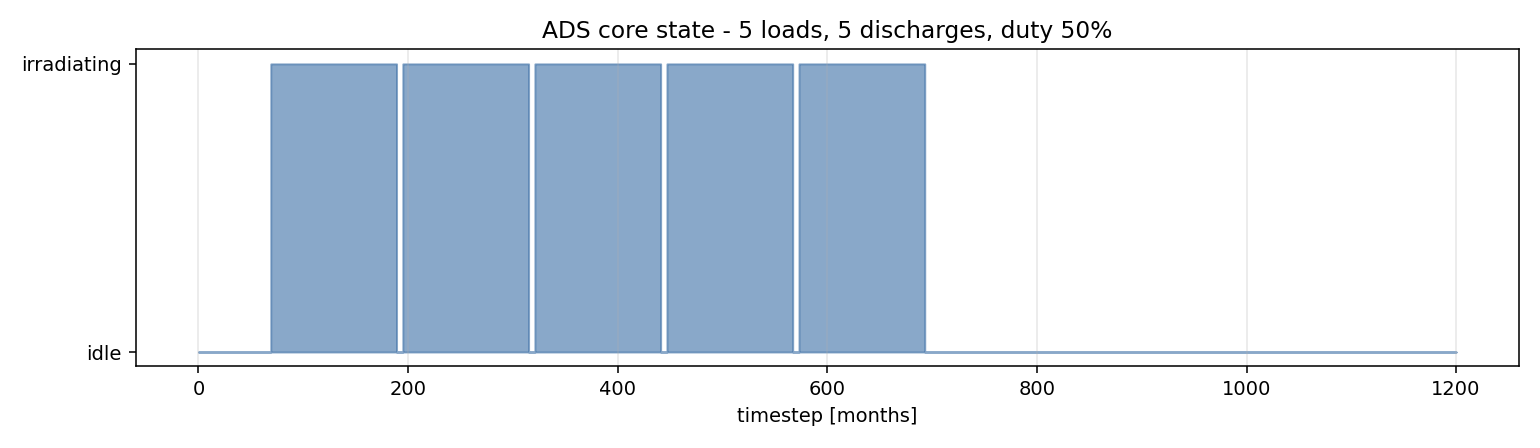
\includegraphics[width=0.95\textwidth]{figures/case3_ma_recycle_100yr_dutycycle}
  \caption[Core state of the minor-actinide-only burner.]{Irradiating-or-idle
  state of the minor-actinide-only core (ADS~1) over the 100-year recycling run.
  The core completes five ten-year cycles and then falls idle because its
  recoverable Np-Am-Cm feed no longer reaches the \(27~\mathrm{t}\) full-core
  loading threshold; the duty factor is \(50\%\).}
  \label{fig:results-case3-recycle-dutycycle}
\end{figure}

\begin{figure}[htbp]
  \centering
  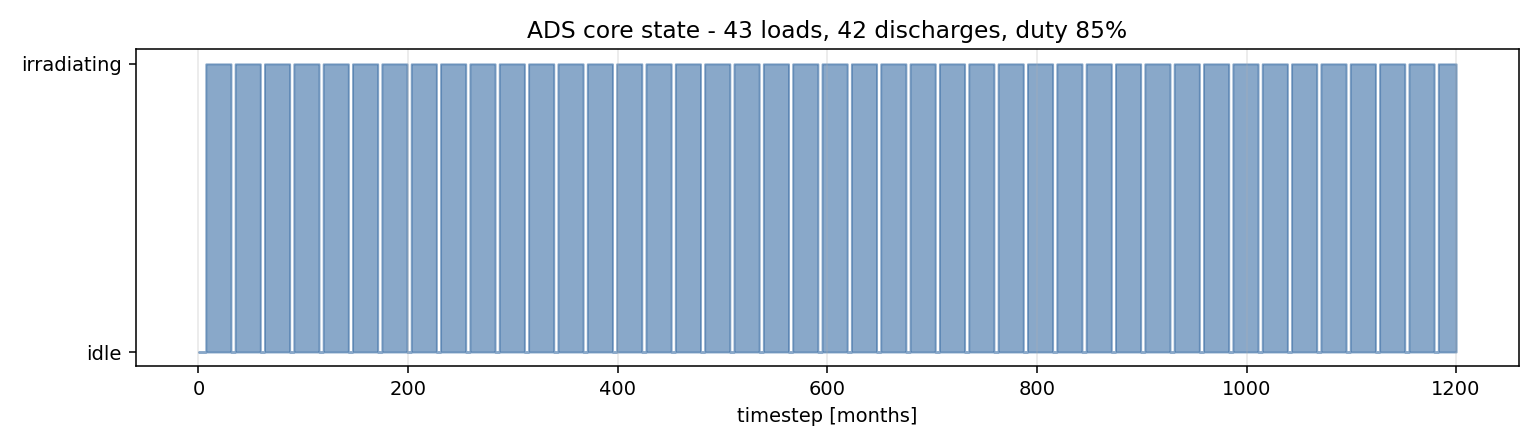
\includegraphics[width=0.95\textwidth]{figures/case4_puma_recycle_100yr_dutycycle}
  \caption[Core state of the \(50/50\) burner.]{Irradiating-or-idle state of the
  \(50/50\) core (ADS~2) over the 100-year recycling run. The small, fast-cycling
  core runs essentially continuously at a duty factor of \(85\%\), sustained by
  the plutonium fraction of its feed.}
  \label{fig:results-case4-recycle-dutycycle}
\end{figure}

For the \(50/50\) core the once-through and recycling runs are indistinguishable,
because the core is cycle-limited: within each two-year cycle there is little
surviving actinide to recover before the next core is due, so recycling changes
almost nothing. This confirms the cycle-limited regime and is why only a single
\(50/50\) run is shown.

\subsection{Recycling versus Once-Through for the Minor-Actinide Core}
\label{subsec:results-ads-recycle}

The minor-actinide-only core is the one configuration where recycling materially
changes the outcome, precisely because it is feed-limited. Comparing the recycling
per-cycle history (Figure~\ref{fig:results-case3-recycle-percycle}) with the
once-through history (Figure~\ref{fig:results-case3-oncethrough-percycle}) isolates
the effect. The two runs share an identical per-cycle signature, the same
\(27~\mathrm{t}\) charge, the same \(11.15~\mathrm{t}\) destroyed, and the same
\(41.3\%\) burn fraction in the bottom panel of each figure, because the reduced-
order depletion physics does not depend on where the feed came from. What differs
is how many cycles the burner completes before its feed is spent: three under
once-through, five under recycling.

The cumulative panels make the consequence concrete. In once-through mode the burner charges \(81~\mathrm{t}\) in total and
records \(33.5~\mathrm{t}\) of net actinide destruction; with recycling it
charges \(135~\mathrm{t}\) and records \(55.8~\mathrm{t}\), an
increase of \(1.67\times\) in actinide destroyed. Recycling achieves this by
recovering the surviving minor actinides from each discharge and returning them to
the feed, so the same atoms make more than one pass through the core and the
burner sustains operation past the point where the once-through supply is spent.

The charged figure is itself the clearest evidence of reuse. The total accessible
minor-actinide inventory is only \(103.8~\mathrm{t}\)
(Section~\ref{sec:results-baseline}), yet the recycling run charges
\(135~\mathrm{t}\), more minor actinide than exists in the national inventory.
This is possible only because recycling returns material for additional passes;
the excess of roughly \(31~\mathrm{t}\) is minor actinide irradiated more than
once. The once-through run, by contrast, charges \(81~\mathrm{t}\), comfortably
within the inventory, and simply stops when the accessible feed is gone.

Even with recycling, however, the burner still stops well short of the horizon.
The initial \(103.8~\mathrm{t}\) minor-actinide inventory is only about
\(3.8\) fresh core-loadings. After each irradiation, only the surviving
neptunium, americium, and curium is eligible to return to the ADS~1 feed; actinide
converted to plutonium is routed outside that feed stream, and the archetype will
not load a partial core. Recycling therefore extends the campaign from three
cores to five, but eventually the recoverable minor-actinide feed remains below
the \(27~\mathrm{t}\) loading threshold.

\begin{figure}[htbp]
  \centering
  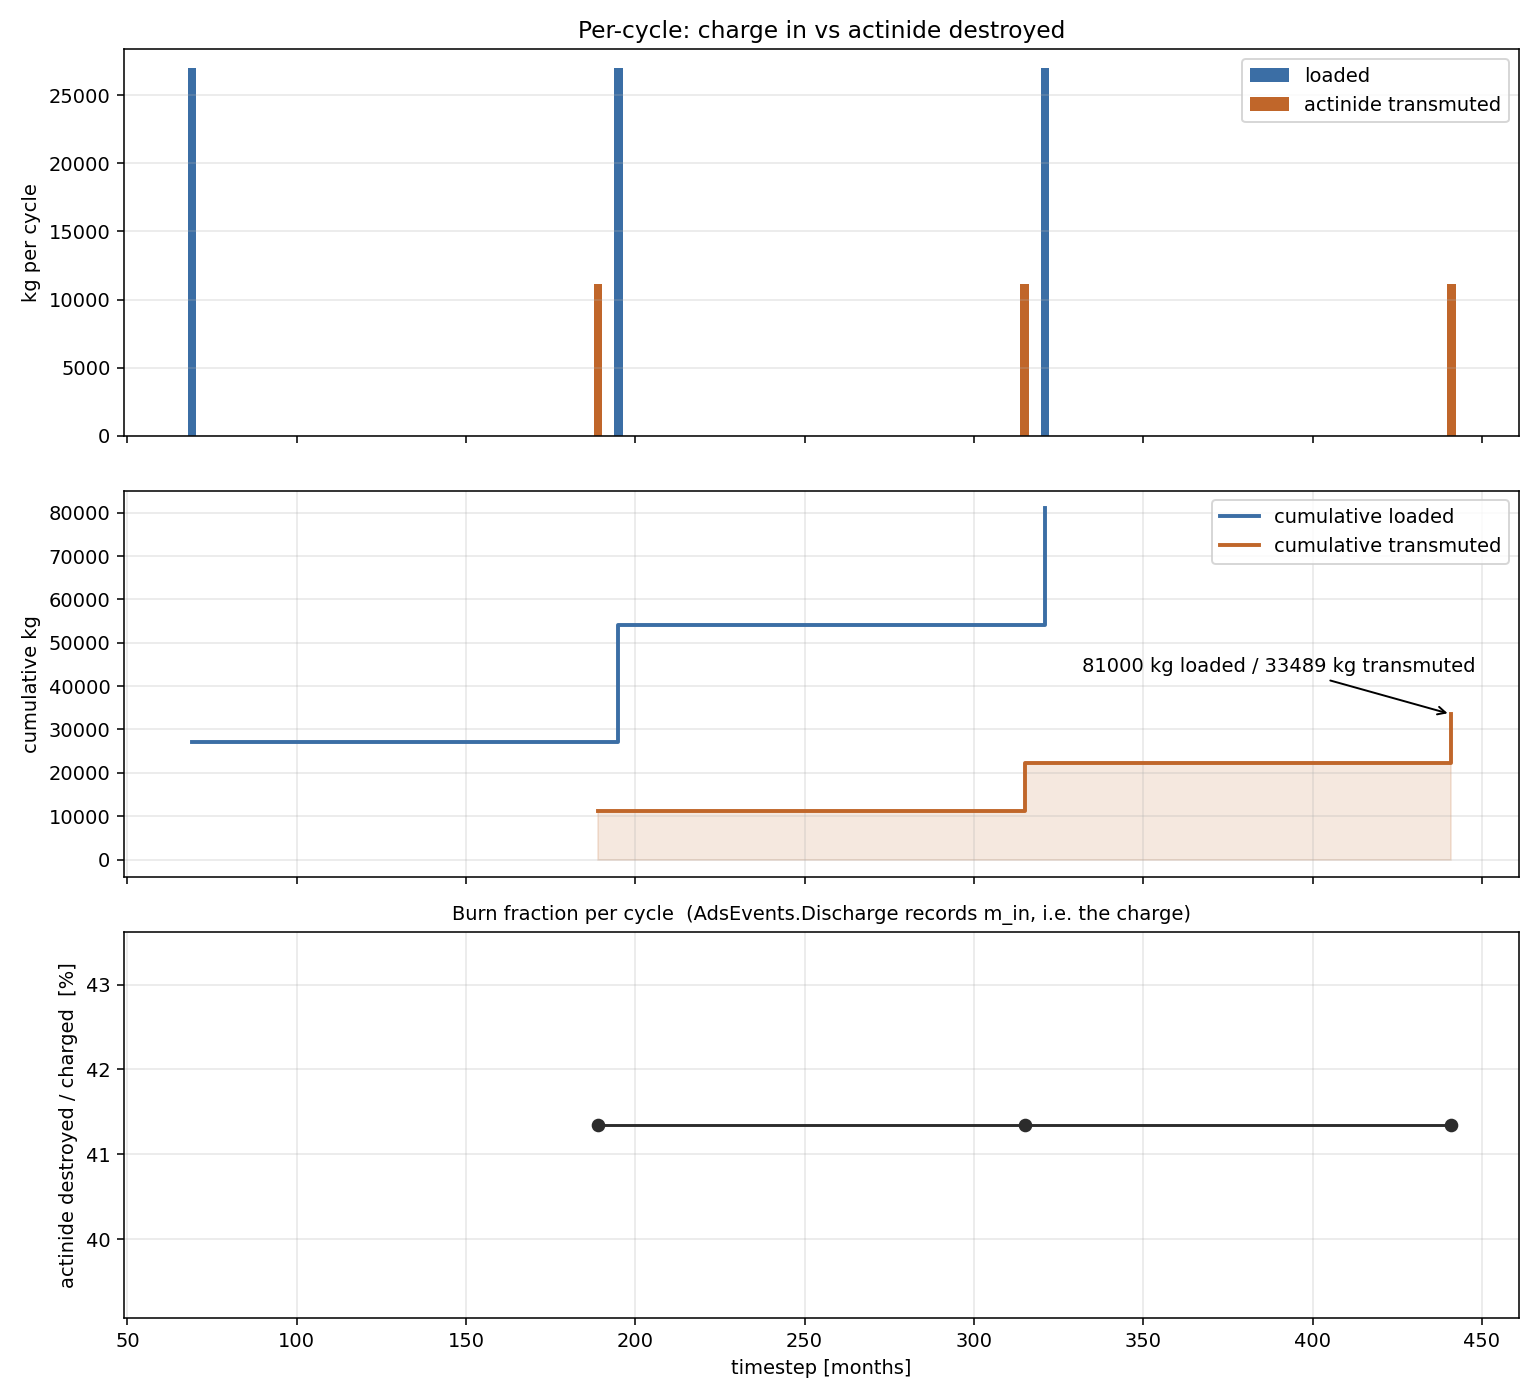
\includegraphics[width=0.95\textwidth]{figures/case3_ma_oncethrough_100yr_percycle}
  \caption[Per-cycle mass accounting for the minor-actinide-only core,
  once-through.]{Per-cycle charge and actinide destruction for the
  minor-actinide-only core (ADS~1), 100-year once-through run. The per-cycle
  charge, destruction, and \(41.3\%\) burn fraction match the recycling run
  (Figure~\ref{fig:results-case3-recycle-percycle}), but the burner completes only
  three cycles, reaching \(81~\mathrm{t}\) charged and \(33.5~\mathrm{t}\)
  of cumulative net actinide destruction before its feed is exhausted.}
  \label{fig:results-case3-oncethrough-percycle}
\end{figure}

\subsection{Transmutation Rate and Mission Scale}
\label{subsec:results-ads-rate}

Taken together, these results frame the scale of the transmutation mission. A
single \(3000~\mathrm{MW_{th}}\) unit destroys actinide at up to about
\(1{,}120~\mathrm{kg\,yr^{-1}}\) at full power, reduced in proportion to its duty
factor. Over a 30-year mission the \(50/50\) core, running near-continuously,
destroys on the order of \(27~\mathrm{t}\) of actinide per unit, while the
minor-actinide-only core destroys less because it stalls once its feed is spent.
The two horizons reinforce this: a cycle-limited core scales its output roughly
linearly with the length of the mission, whereas a feed-limited core plateaus once
the accessible inventory is consumed, which is why extending the minor-actinide
core from 30 to 100 years adds only two further cycles.

The consequence is that sizing a fleet to destroy the minor-actinide inventory is
not the usual reactor-capacity problem. The entire national minor-actinide
inventory is under four core-loadings; the limitation is how quickly that finite
inventory can be retrieved, separated, and, critically, recycled, not how much
reactor power is installed. Additional units shorten the calendar time to work
through the available feed but cannot destroy more minor actinide than the
inventory contains. A configuration that instead co-burns plutonium, as the
\(50/50\) core does, sidesteps the feed limit but redefines the mission from
minor-actinide destruction to bulk transuranic destruction. This inversion of the
usual sizing question, feed-bound rather than power-bound, is the central
practical finding of the transmutation results, and it is examined further in the
discussion of Section~\ref{sec:results-discussion}.


%%%%%%%%%%%%%%%%%%%%%%%%%%%%%%%%%%%%%%%%%%%%%%%%%%%%%%%%%%%%%%%%%%%%%%%%%%%%%%%%%%%%%%%%%%%%%%%%%%%%%%%%%%%%%%%%%%%%%%%%%%%%%%%%%
%%%%%%%%%%%%%%%%%%%%%%%%%%%%%%%%%%%%%%%%%%%%%%%%%%%%%%%%%%%%%%%%%%%%%%%%%%%%%%%%%%%%%%%%%%%%%%%%%%%%%%%%%%%%%%%%%%%%%%%%%%%%%%%%%
%%%%%%%%%%%%%%%%%%%%%%%%%%%%%%%%%%%%%%%%%%%%%%%%%%%%%%%%%%%%%%%%%%%%%%%%%%%%%%%%%%%%%%%%%%%%%%%%%%%%%%%%%%%%%%%%%%%%%%%%%%%%%%%%%

\section{Processed Inventory}
\label{sec:results-evolution}

The transmutation results of Section~\ref{sec:results-ads} describe what the
burner does per cycle; this section follows the material through the whole fuel
cycle and asks what becomes of the national inventory once it is processed. Every
kilogram drawn from \texttt{us\_inventory} meets one of three fates: it is
destroyed by fission in the \gls{ADS}, it is recovered and returned to the feed
under recycling, or it is routed to disposal. Tracking these streams shows both
what the mission accomplishes and what it leaves behind, and connects the results
back to the waste-management motivation of Chapter~\ref{ch:background}.

\subsection{Disposition of the Minor-Actinide Inventory}
\label{subsec:results-fate-ma}

Table~\ref{tab:results-ma-fate} closes the actinide mass balance against the
\(103.8~\mathrm{t}\) of minor actinide initially present in the accessible
inventory (Section~\ref{sec:results-baseline}). The quantity labeled
``undestroyed descendant actinide'' is the initial actinide mass minus the net
actinide destruction recorded by the ADS. It is therefore not equivalent to
minor-actinide feed still available to the burner: it includes any surviving
neptunium, americium, and curium, actinides produced by transmutation such as
plutonium, material routed to waste, and material held in facility buffers.

In once-through operation the burner records \(33.5~\mathrm{t}\) of net actinide
destruction and leaves \(70.3~\mathrm{t}\) of descendant actinide undestroyed. Of
that remainder, roughly \(47.5~\mathrm{t}\) is surviving actinide discharged to
waste, while about \(22.8~\mathrm{t}\) remains in unprocessed inventory because
it is insufficient to form another \(27~\mathrm{t}\) core.

With recycling, net actinide destruction increases to \(55.8~\mathrm{t}\), leaving
\(48.0~\mathrm{t}\) of descendant actinide somewhere in the modeled fuel cycle.
The \(48.0~\mathrm{t}\) value does not imply that a further \(27~\mathrm{t}\)
minor-actinide core could be loaded. In the ADS~1 flowsheet, only Np, Am, and Cm
are recovered as burner feed; plutonium produced during irradiation is routed
outside the minor-actinide feed stream, and the remaining recoverable
minor-actinide inventory is distributed among products and buffers. The ADS
therefore stalls when its feed buffer cannot again accumulate a full
\(27~\mathrm{t}\) loading.

\begin{table}[htbp]
    \centering
    \caption{Actinide mass balance relative to the \(103.8~\mathrm{t}\) of minor
    actinide initially present in the accessible inventory at the end of the
    100-year minor-actinide-only runs. ``Undestroyed descendant actinide''
    includes surviving minor actinides, actinides produced by transmutation,
    material routed to waste, and material held in facility buffers; it is not
    the mass of usable minor-actinide feed remaining.}
    \label{tab:results-ma-fate}
    \begin{tabular}{p{0.42\textwidth} p{0.22\textwidth} p{0.22\textwidth}}
        \hline
        \textbf{Disposition} & \textbf{Once-through} & \textbf{Recycle} \\
        \hline
        Net actinide destruction          & \(33.5~\mathrm{t}\) & \(55.8~\mathrm{t}\) \\
        Undestroyed descendant actinide     & \(70.3~\mathrm{t}\) & \(48.0~\mathrm{t}\) \\
        \hline
        Initial accessible MA inventory     & \(103.8~\mathrm{t}\) & \(103.8~\mathrm{t}\) \\
        \hline
    \end{tabular}
\end{table}

\subsection{Composition of the Waste Stream}
\label{subsec:results-fate-waste}

Figure~\ref{fig:results-case3-recycle-waste} shows the final composition of the
waste repository for the minor-actinide-only recycling run, as the mass of each of
the 25 most abundant nuclides. The stream is overwhelmingly uranium: \({}^{238}\mathrm{U}\)
alone accounts for roughly \(8.5\times10^{4}~\mathrm{t}\), four orders of magnitude
above any minor actinide. This is a direct consequence of the scarcity documented
in Section~\ref{sec:results-baseline}. Because minor actinide is only about
\(0.12\%\) of the spent fuel, extracting the roughly \(100~\mathrm{t}\) the burner
consumes requires separations to process on the order of the entire drawn
inventory, tens of thousands of tonnes of spent fuel, and the uranium and fission
products stripped from that fuel dominate the disposal stream. The mass sent to
disposal is therefore not reduced by the transmutation mission; it is only changed
in character.

That change in character is nonetheless the intended effect, and it is visible in
the figure. Minor actinides are almost absent from the waste: americium, the most
abundant minor actinide in the original fuel, does not appear among the major
waste nuclides at all under recycling, having been recovered and burned. In the
once-through run the same plot shows a small residual \({}^{241}\mathrm{Am}\) peak,
which recycling removes, a direct illustration of recovery closing that pathway.
The minor-actinide-only cycle thus succeeds in stripping minor actinide from the
waste, but does not reduce its volume.

The figure also exposes the principal limitation of the minor-actinide-only
configuration. Plutonium is the second-largest component of the waste, with
\({}^{239}\mathrm{Pu}\) near \(7\times10^{2}~\mathrm{t}\): because this burner
consumes only minor actinide, separations routes the entire plutonium content of
every processed assembly straight to disposal, untouched. A cycle designed to
destroy minor actinide therefore leaves the larger and equally long-lived
plutonium inventory in the waste, which is precisely the gap the \(50/50\)
configuration is meant to address.

\begin{figure}[htbp]
  \centering
  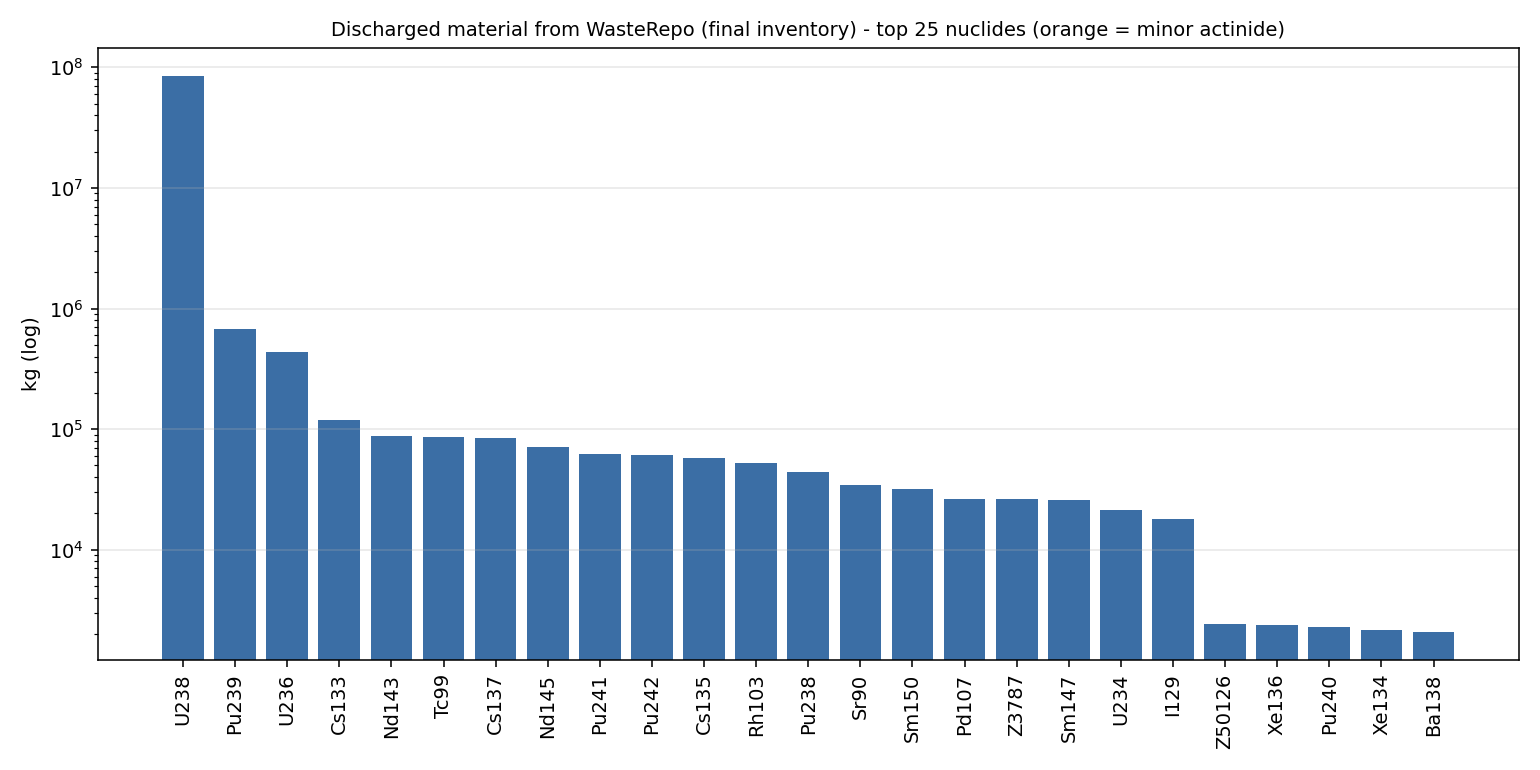
\includegraphics[width=0.95\textwidth]{figures/case3_ma_recycle_100yr_waste_composition}
  \caption[Waste-stream composition for the minor-actinide-only core.]{Final
  waste-repository composition for the minor-actinide-only recycling run (ADS~1),
  showing the 25 most abundant nuclides on a logarithmic mass scale; minor
  actinides are highlighted. The stream is dominated by uranium and plutonium
  stripped by separations, while minor actinides are nearly absent, having been
  recovered and burned.}
  \label{fig:results-case3-recycle-waste}
\end{figure}

\subsection{Material Recovered under Recycling}
\label{subsec:results-fate-recovered}

Where the minor-actinide-only cycle sends plutonium to waste, the \(50/50\)
configuration returns it to the feed. Figure~\ref{fig:results-case4-recycle-product}
shows the material discharged from the \gls{ADS} in the \(50/50\) recycling run,
which separations recovers and blends back into fresh feed. The stream is led by
plutonium isotopes, surviving and bred \({}^{239}\mathrm{Pu}\),
\({}^{238}\mathrm{Pu}\), and \({}^{240}\mathrm{Pu}\), followed by the minor
actinides \({}^{237}\mathrm{Np}\), \({}^{244}\mathrm{Cm}\), \({}^{241}\mathrm{Am}\),
and their heavier companions, alongside the fission products of the cycle. By
recovering the plutonium as well as the minor actinides, the \(50/50\) cycle keeps
that plutonium in the burner over successive passes rather than stranding it in
waste, which is why it addresses the broader transuranic inventory rather than the
minor actinides alone. The presence of \({}^{242\mathrm{m}}\mathrm{Am}\) in the
recovered stream also confirms that the archetype preserves the metastable state
through the composition transformation, rather than collapsing it onto the ground
state.

\begin{figure}[htbp]
  \centering
  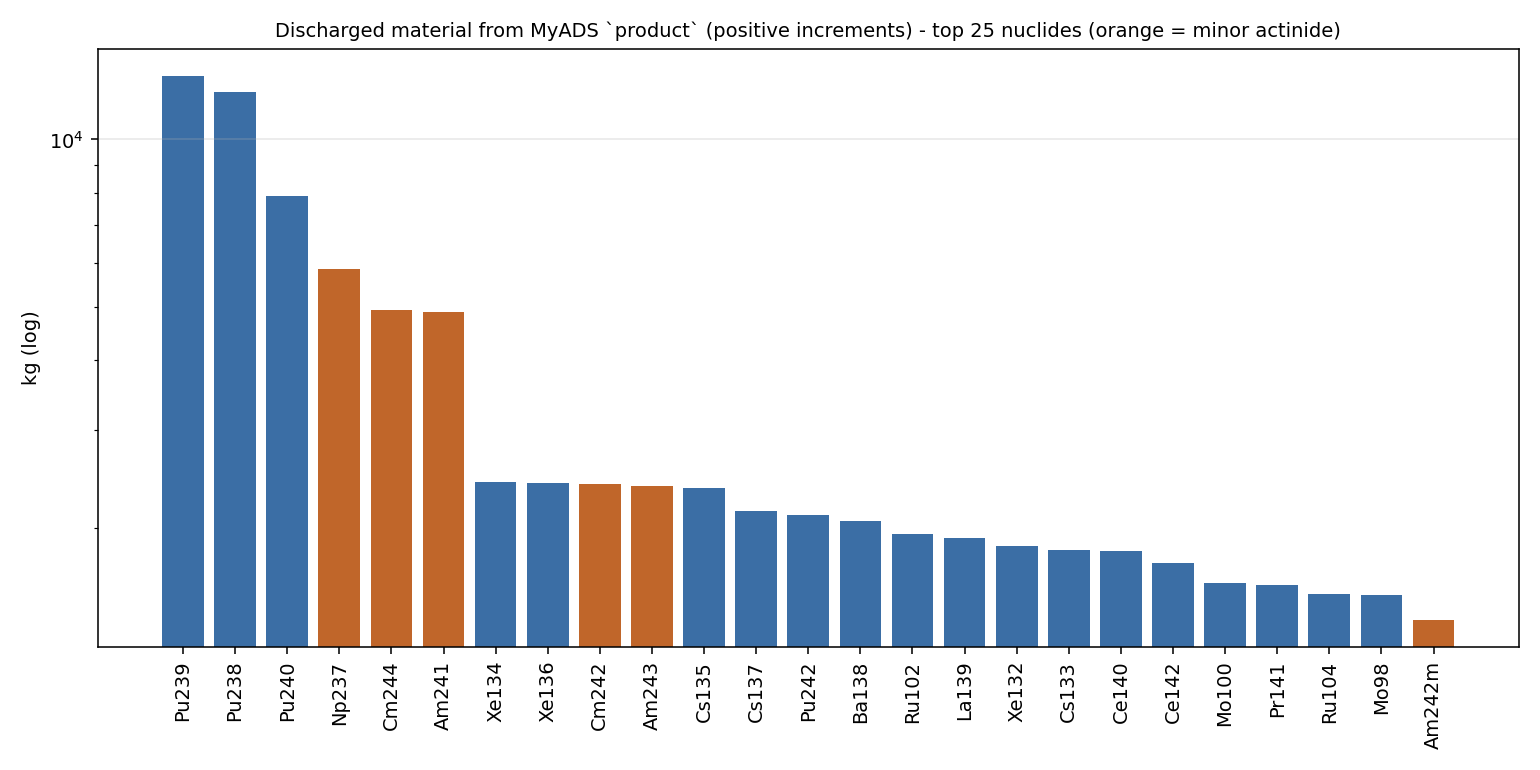
\includegraphics[width=0.95\textwidth]{figures/case4_puma_recycle_100yr_ads_product}
  \caption[Recovered discharge stream for the \(50/50\) core.]{Composition of the
  material discharged from the \gls{ADS} in the \(50/50\) recycling run (ADS~2),
  showing the 25 most abundant nuclides on a logarithmic mass scale; minor
  actinides are highlighted. Plutonium leads the recovered stream, followed by the
  minor actinides and fission products, all of which recycling returns to the
  feed.}
  \label{fig:results-case4-recycle-product}
\end{figure}

\subsection{Implications for the Waste Inventory}
\label{subsec:results-fate-implications}

Taken together, these results qualify what transmutation achieves for the national
inventory. Over a century, even the more favorable recycling configuration
destroys only about half of the accessible minor actinide, and it does so at the
cost of processing essentially the entire spent-fuel inventory, the bulk of which, 
uranium, fission products, and, for the minor-actinide-only cycle, plutonium, 
still requires disposal. The mission changes the isotopic character of the waste
by removing minor actinide, which is the component that dominates its long-term
radiotoxicity and heat load; it does not substantially reduce the bulk material mass requiring management
and disposal. Quantifying the resulting reduction in radiotoxicity or decay heat
would require coupling these mass histories to a decay and dose calculation, which
is beyond the scope of this work but is a natural extension of it
(Chapter~\ref{ch:conclusion}). What the fuel-cycle results establish is the
upstream reality any such benefit must be weighed against: minor-actinide
transmutation is constrained not by reactor performance but by the scarcity of its
feed and the scale of the inventory that must be handled to extract it.


%%%%%%%%%%%%%%%%%%%%%%%%%%%%%%%%%%%%%%%%%%%%%%%%%%%%%%%%%%%%%%%%%%%%%%%%%%%%%%%%%%%%%%%%%%%%%%%%%%%%%%%%%%%%%%%%%%%%%%%%%%%%%%%%%
%%%%%%%%%%%%%%%%%%%%%%%%%%%%%%%%%%%%%%%%%%%%%%%%%%%%%%%%%%%%%%%%%%%%%%%%%%%%%%%%%%%%%%%%%%%%%%%%%%%%%%%%%%%%%%%%%%%%%%%%%%%%%%%%%
%%%%%%%%%%%%%%%%%%%%%%%%%%%%%%%%%%%%%%%%%%%%%%%%%%%%%%%%%%%%%%%%%%%%%%%%%%%%%%%%%%%%%%%%%%%%%%%%%%%%%%%%%%%%%%%%%%%%%%%%%%%%%%%%%

\section{Discussion}
\label{sec:results-discussion}

The results of this chapter can be read as a single argument about scale. The
\texttt{us\_inventory} and \texttt{ads} archetypes were built to connect a
detailed, assembly-resolved picture of the U.S. spent-fuel inventory to a
reduced-order model of an accelerator-driven burner, and running them together
turns qualitative expectations about minor-actinide transmutation into quantified
constraints. Two findings dominate, and both point the same way.

\subsection{The Mission is Feed-Bound}
\label{subsec:discussion-feedbound}

The central result is that a minor-actinide transmutation mission is limited by
the availability of its feed rather than by installed reactor capacity. The
accessible minor-actinide inventory is \(103.8~\mathrm{t}\), under four loadings
of a single \(27~\mathrm{t}\) core, so the binding question is not how much power
can be deployed but how quickly that finite, dilute inventory can be retrieved,
separated, and recycled. The minor-actinide-only core makes this concrete: it is
feed-limited, stalling after three cores once-through or five with recycling
(Section~\ref{subsec:results-ads-recycle}), and no increase in reactor power can
change that, because the feed to sustain further cores does not exist. This
inverts the usual framing of a reactor deployment, in which capacity is the
constraint and fuel is assumed abundant.

A simple rate calculation frames the fleet question that follows from this. A
\(3000~\mathrm{MW_{th}}\) unit destroys actinide at up to about
\(1{,}120~\mathrm{kg\,yr^{-1}}\) at full power
(Section~\ref{subsec:results-ads-rate}), so clearing the \(103.8~\mathrm{t}\)
inventory represents on the order of \(90\) unit-years of full-power operation.
Distributed over a 30-year mission this is roughly three units' worth of
destruction capacity; a single unit would require most of a century, and the
feed-limited minor-actinide core cannot in practice run at full duty for that long.
This is not a precise fleet-sizing, it omits reprocessing losses, retrieval and
transport logistics, and the duty-factor penalty the feed limit itself imposes, but
it establishes the order of magnitude: the transmutation of the national
minor-actinide inventory is a task for a handful of high-power units over decades,
and its pace is set by fuel handling rather than by how many units are built.

The \(50/50\) configuration escapes the feed limit, but only by changing the
mission. By co-burning plutonium, ten times more abundant in the inventory than
minor actinide, the small, fast-cycling core stays fed for the full century at a
\(85\%\) duty factor and destroys \(91.8~\mathrm{t}\) of actinide, far more than the
minor-actinide core's \(55.8~\mathrm{t}\)
(Section~\ref{subsec:results-ads-cases}). But roughly half of that is plutonium, so
the \(50/50\) core is a transuranic burner rather than a minor-actinide burner. The
choice between the two configurations is therefore a choice of mission: destroy the
scarce, high-radiotoxicity minor actinides at a pace bounded by their scarcity, or
destroy the broader transuranic inventory at a higher rate by accepting plutonium
as feed.

\subsection{Transmutation Changes Waste Composition}
\label{subsec:discussion-character}

The second finding concerns what the mission does to the waste. Because minor
actinide is only \(0.12\%\) of the spent fuel, extracting the roughly
\(100~\mathrm{t}\) the burner consumes requires separations to process on the order
of the entire drawn inventory, and the uranium, fission products, and, for the
minor-actinide-only cycle, plutonium stripped from that fuel dominate the disposal
stream (Section~\ref{subsec:results-fate-waste}). The transmutation mission produces
little reduction in the total bulk mass
routed to waste. Its principal modeled effect is instead a change in isotopic
composition through the destruction and redistribution of actinides.
Repository volume, package requirements, and disposal-footprint effects were
not evaluated in this work. It removes minor actinide, the component that dominates
the long-term radiotoxicity and decay heat of spent fuel. That is a meaningful
outcome for repository performance, but it is a qualitative change to the waste
rather than a reduction of it, and it is bought at the cost of handling the full
inventory.

This reframes the value proposition of transmutation in a way the fuel-cycle model
is well suited to expose. The benefit is not less waste but longer-lived
constituents removed from it; the cost is a fuel cycle that must retrieve,
transport, and reprocess essentially the entire national inventory to recover a
trace component. Whether that trade is worthwhile is a question about repository
requirements and reprocessing capacity, not about the burner itself.

\subsection{Limitations}
\label{subsec:discussion-limitations}

Several limitations bound the interpretation of these results, and identifying them
also marks the most useful directions for further work.

The \gls{ADS} model is reduced-order. The burner does not solve neutron transport
during the simulation; it reads precomputed \textsc{Serpent} depletion cases and
selects and interpolates among them (Section~\ref{sec:ads-archetype}). This is
appropriate for a fuel-cycle study, where the quantity of interest is the mass
transmuted per core rather than the detailed in-core physics, and the per-cycle
rate was shown to agree with an independent fission-energy balance to within a few
percent (Section~\ref{subsec:results-ads-burn}). But it inherits the assumptions of
the underlying cases, a single homogeneous fuel region, a fixed geometry, and a
library spanning only the two representative feeds used here, and it cannot capture
behavior outside the tabulated cases. A core whose composition drifts far from any
library case is matched to the nearest one rather than modeled directly, and the
constant per-cycle burn fraction is a consequence of irradiating every core to the
same point on the same trajectory, not a physical invariant.

The inventory-selection results characterize the feed directly from the static
inventory rather than from the coupled simulation
(Section~\ref{sec:results-policy}). This is exact, because the selection is a
deterministic ordering of a fixed pool, but it means the policy comparison isolates
the supply side and does not reflect any feedback between selection and burner
operation. All production scenarios use the single \texttt{highest\_minor\_actinide}
policy, so the effect of policy on full-cycle outcomes, as opposed to on the feed,
is left for future work.

Finally, the study stops at the mass balance. It quantifies what is destroyed and
what remains but does not evaluate the radiological or economic consequences that
determine whether the mission is worthwhile. Radioactive decay is modeled within
the simulation, so material compositions are aged as they move through the fuel
cycle; but no downstream radiotoxicity or decay-heat calculation is applied to the
final waste compositions, so the reduction in long-term radiological hazard that
motivates minor-actinide removal is not quantified here. Likewise, no cost,
facility, or transportation model accompanies the fuel cycle, so the substantial
reprocessing and handling burden the results imply is described but not priced.Nor does the model
represent the retrieval and transport logistics that the provenance results
(Section~\ref{subsec:results-policy-provenance}) are designed to feed. These are not
incidental omissions but the natural next steps: the assembly-resolved provenance,
the mass-conserving discharge streams, and the feed-limited operating histories
developed here are precisely the inputs a subsequent radiotoxicity, economic, or
siting analysis would require, and building those couplings onto this framework is
the direction the concluding chapter identifies
(Chapter~\ref{ch:conclusion}).